\documentclass[conference]{IEEEtran}
\IEEEoverridecommandlockouts

% ==========================================
% PACKAGES
% ==========================================
\usepackage{cite}
\usepackage{amsmath,amssymb,amsfonts}
\usepackage{algorithmic}
\usepackage{algorithm}
\usepackage{graphicx}
\usepackage{textcomp}
\usepackage{xcolor}
\usepackage{booktabs}
\usepackage{multirow}
\usepackage{url}
\usepackage{float}

% --- TIKZ & PLOTS ---
\usepackage{tikz}
\usetikzlibrary{shapes.geometric, arrows, positioning, fit, calc, backgrounds, shadows}

% --- FORMATTING CONFIGURATION ---
\def\BibTeX{{\rm B\kern-.05em{\sc i\kern-.025em b}\kern-.08em
    T\kern-.1667em\lower.7ex\hbox{E}\kern-.125emX}}

% Ensure strict formatting for "Capstone" feel
\setlength{\parskip}{0.5em}

\begin{document}

% ==========================================
% TITLE
% ==========================================
\title{Architectural Irreversibility: Enforcing Privacy, Governance, and Trust in Intelligent Campus Systems}

% ==========================================
% AUTHOR
% ==========================================
\author{\IEEEauthorblockN{Narendra Babu P}
\IEEEauthorblockA{\textit{Department of Computer Science} \\
\textit{Swarnandhra College of Engineering \& Technology}\\
Narsapur, India \\
narendrababu.p@swarnandhra.ac.in}
}

\maketitle

% ==========================================
% ABSTRACT
% ==========================================
\begin{abstract}
As intelligent systems permeate educational environments, the tension between safety analytics and individual privacy has reached a critical breaking point. Traditional ``Privacy-by-Policy'' approaches---relying on encryption, access controls, and post-hoc audits---fail to mitigate the structural risks of surveillance-centric architectures. This paper introduces \textit{Architectural Irreversibility} as a foundational design paradigm. We propose ``ScholarMasterEngine,'' an eight-layer system where privacy is enforced not by regulation, but by the architecture of the data pipeline. By utilizing one-way data transformations, mandatory runtime governance gates, and visible trust indicators, the system renders pixel-space reconstruction of sensitive biometric data structurally underdetermined. We demonstrate that durable trust in intelligent systems requires structural constraints that reduce reliance on institutional intent, achievable only when the capability to persist raw biometric data is architecturally eliminated.
\end{abstract}

\begin{IEEEkeywords}
Architectural Irreversibility, Automated Stewardship, Privacy-by-Design, Edge AI, Trusted Systems.
\end{IEEEkeywords}

% ==========================================
% SECTION 0: POSITIONING STATEMENT
% ==========================================
\section*{Positioning Statement}
Contemporary intelligent campus systems promise safety, efficiency, and insight, yet repeatedly fail to achieve social legitimacy. Despite widespread deployment of encryption, access controls, audit logs, and regulatory compliance frameworks, these systems continue to provoke resistance, anxiety, and distrust from the very populations they claim to serve. This failure is not incidental; it is structural. This work is rigorously aligned with the Unified Reference Model \cite{P20} and adheres to the Formal Foundations of Distributed Trust \cite{P21} established for the ScholarMaster architecture.

Most privacy-preserving AI systems are built atop surveillance-centric architectures. Raw sensory data---images, audio, identifiers---are captured, persisted, and analyzed first, while governance, consent, and accountability are applied later as external controls. In such systems, privacy is treated as a policy obligation rather than a system property. This approach assumes that misuse can be prevented through regulation, oversight, or operator discipline. History demonstrates the opposite: if sensitive data exists, it will eventually be repurposed, leaked, inferred, or abused.

This work argues that privacy failures are architectural, not legal. Post-hoc governance cannot reliably constrain systems whose core data flows already encode surveillance assumptions. Audits detect violations after harm occurs. Policies regulate behavior but do not eliminate capability. Transparency reports explain systems that should not have existed in their current form. As a result, trust collapses---not because users misunderstand the technology, but because they correctly perceive the asymmetry of power embedded within it.

We propose a different premise: privacy must be enforced before information exists, not after it is collected. This requires rethinking intelligent systems as irreversible pipelines rather than reversible data processors. Once raw sensory input is transformed into non-reconstructable abstractions and the originals are destroyed, entire classes of raw-data privacy risk are eliminated---not mitigated, not regulated, but made structurally underdetermined.

However, technical irreversibility alone is insufficient for social acceptance. Even mathematically sound constraints fail if they remain invisible to those affected. Trust is not established by cryptographic proofs hidden in documentation; it emerges when system limits are directly observable. A system that claims restraint but visually behaves like surveillance will be treated as surveillance. Conversely, a system that visibly demonstrates what it cannot see, store, or infer enables users to verify privacy claims without specialized expertise.

This capstone introduces \textbf{Architectural Irreversibility} as a foundational design principle for intelligent campus systems, coupled with mandatory runtime governance and visible privacy mechanisms that transform trust from an assumption into an observable system output. Rather than adding privacy as a feature, the system eliminates the conditions under which raw biometric privacy violations could occur. Rather than relying on institutional assurances, it exposes its own constraints in real time.

The contribution of this work is not a new detection model, dataset, or optimization technique. It is a system-level reframing: a demonstration that intelligent environments can be designed such that raw data persistence and pixel-space misuse are structurally precluded, governance is non-bypassable, and trust is continuously verifiable. In doing so, this work challenges the prevailing assumption that surveillance is the unavoidable substrate of intelligent systems and presents an alternative category---\textbf{Automated Stewardship}---in which intelligence and dignity are not in conflict. This paper does not evaluate performance, hardware resilience, or economic cost; those analyses are provided in Papers 10 and 11. The focus here is architectural necessity and formal constraint.

% ==========================================
% 1. PROBLEM REFRAMING
% ==========================================
\section{Problem Reframing: Why Privacy-by-Policy Fails}

\subsection{The False Promise of Post-Hoc Privacy}
Most intelligent campus systems claim privacy compliance through a familiar toolbox: encryption at rest, role-based access control, audit logging, consent forms, and regulatory alignment (e.g., GDPR, DPDP). These mechanisms are widely presented as sufficient safeguards against misuse. Yet empirical evidence from education, healthcare, and smart-city deployments shows persistent distrust, resistance, and chilling effects even in systems that are technically compliant.

The core failure is categorical. These protections operate after sensitive information has already been captured, retained, or processed in reversible form. Encryption secures data that already exists. Access controls govern who may use data that already exists. Audit logs record actions taken on data that already exists. Consent governs permission to process data that already exists. None of these mechanisms alter the fundamental fact that the system possesses high-fidelity representations of individuals.

From a systems perspective, this is a critical flaw: capability precedes governance. Once a system can see, store, or infer sensitive attributes, no policy can reliably ensure that this capability will never be exercised incorrectly---whether through error, misconfiguration, adversarial compromise, or future repurposing. Privacy-by-policy assumes that future behavior can be perfectly constrained. Architectural history repeatedly disproves this assumption.

\subsection{Capability Leakage as an Inevitable Outcome}
In surveillance-derived architectures, sensitive data persistence creates latent capability. Even if unused today, the mere availability of raw frames, embeddings, or identifiers enables secondary inference tomorrow. Models can be retrained. Logs can be re-queried. Correlations can be rediscovered. What begins as attendance monitoring becomes behavioral profiling; what begins as safety analytics becomes performance surveillance.

This phenomenon---\textit{capability leakage}---is not malicious by default. It arises naturally from software evolution. New features are added. New stakeholders request access. New analytics promise value. Each step appears locally reasonable, yet globally transforms the system's role. Privacy erosion occurs incrementally and often invisibly to users, who experience only the cumulative effect.

Crucially, users intuit this risk correctly. Resistance to monitoring systems is often mischaracterized as irrational fear or lack of technical understanding. In reality, it is a rational response to architectures that concentrate asymmetric power while offering only procedural assurances. When a system can see more than it admits, trust collapses regardless of stated intent.

\subsection{The Limits of Compliance-Driven Design}
Regulatory frameworks are frequently invoked as evidence of safety. However, regulations govern use, not existence. They specify lawful purposes, retention periods, and user rights, but they do not---and cannot---mandate architectural impossibility. A compliant system may still collect high-resolution biometric data, store it securely, and promise deletion later. From a legal standpoint this may suffice; from a systems standpoint it does not.

Moreover, compliance is temporally fragile. Laws change. Interpretations shift. Jurisdictions differ. A system architected around maximal data retention with minimal policy constraints can become non-compliant overnight---or worse, remain compliant while violating emerging social norms. Designing privacy as a legal afterthought ties system legitimacy to external institutions rather than to intrinsic structural constraints.

\subsection{Trust as a Systems Property}
Trust is often framed as a human factors problem: users must be educated, interfaces improved, consent clarified. While these measures are valuable, they cannot compensate for architectures that contradict their own assurances. Trust cannot be demanded, trained, or marketed into existence. It emerges when system behavior is verifiable and aligned with user expectations.

In surveillance-centric systems, users are asked to trust intent. In contrast, robust systems enable users to trust structure. If a system cannot technically store raw frames, then direct biometric misuse becomes structurally precluded. If identity cannot be reconstructed from outputs, discrimination becomes structurally constrained. If governance cannot be bypassed at runtime, accountability is no longer aspirational.

This reframing leads to a central claim of this work: this work argues that durable trust in intelligent systems requires structural constraints that reduce reliance on institutional intent.

\subsection{Reframing the Design Question}
The prevailing design question in intelligent environments has been:
\textit{``How do we collect useful data while complying with privacy requirements?''}

This work proposes a different question:
\textit{``How do we design systems such that collecting harmful data is structurally precluded in the first place?''}

Answering this question requires abandoning the assumption that raw sensory fidelity is necessary for intelligence. It requires privileging irreversible transformations over reversible storage, mandatory governance over optional policy, and observable constraints over hidden assurances.

% ==========================================
% 2. ARCHITECTURAL IRREVERSIBILITY
% ==========================================
\section{Architectural Irreversibility}

\subsection{From Reversible Pipelines to Irreversible Systems}
Most AI systems are architected as reversible pipelines. Raw inputs are ingested, transformed, stored, and reprocessed as needed. Even when intermediate representations are abstracted, the original data often persists---on disk, in memory, in logs, or in backups. This reversibility is convenient for debugging, retraining, and feature expansion, but it is fundamentally incompatible with strong structural privacy constraints.

Architectural irreversibility rejects this paradigm. An irreversible system is one in which certain transformations are destructive by design: once applied, the original information cannot be reconstructed, queried, or recovered.

% --- FIGURE 1: IRREVERSIBILITY PIPELINE ---
\begin{figure}[htbp]
\centering
\resizebox{\columnwidth}{!}{
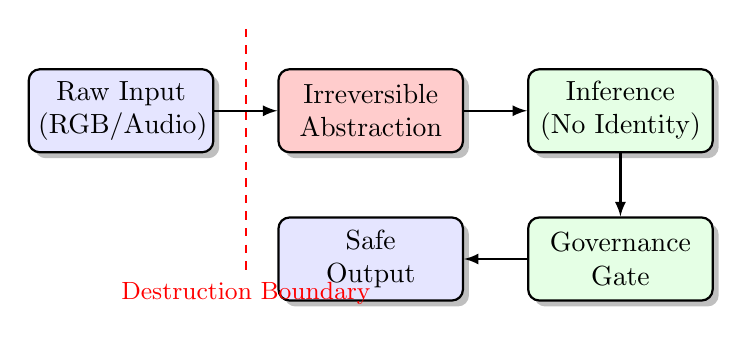
\begin{tikzpicture}[node distance=1.5cm, auto, >=latex, thick]
    % Styles
    \tikzstyle{block} = [rectangle, draw, fill=blue!10, text width=6em, text centered, rounded corners, minimum height=3em, drop shadow]
    \tikzstyle{destruct} = [rectangle, draw, fill=red!20, text width=6em, text centered, rounded corners, minimum height=3em, drop shadow]
    \tikzstyle{safe} = [rectangle, draw, fill=green!10, text width=6em, text centered, rounded corners, minimum height=3em, drop shadow]
    \tikzstyle{line} = [draw, -latex, thick]

    % Nodes
    \node [block] (input) {Raw Input\\(RGB/Audio)};
    \node [destruct, right=0.8cm of input] (destroy) {Irreversible\\Abstraction};
    \node [safe, right=0.8cm of destroy] (infer) {Inference\\(No Identity)};
    \node [safe, below=0.8cm of infer] (govern) {Governance\\Gate};
    \node [block, left=0.8cm of govern] (output) {Safe\\Output};

    % Edges
    \draw [line] (input) -- (destroy);
    \draw [line] (destroy) -- (infer);
    \draw [line] (infer) -- (govern);
    \draw [line] (govern) -- (output);

    % Barrier
    \draw [red, dashed, thick] ($(input.north east)+(0.4,0.5)$) -- ($(input.south east)+(0.4,-1.5)$) node [at end, below, text=red, font=\small] {Destruction Boundary};
\end{tikzpicture}
}
\caption{The Irreversible Pipeline. Raw data exists only transiently in L1/L2 and is destroyed at the boundary before inference occurs. No path exists to recover the input.}
\label{fig:pipeline}
\end{figure}

\subsection{Irreversibility vs. Anonymization}
It is critical to distinguish irreversibility from commonly cited privacy techniques:
\begin{itemize}
    \item \textbf{Anonymization:} Removes explicit identifiers but preserves rich signals allowing re-identification.
    \item \textbf{Pseudonymization:} Replaces identifiers with tokens, enabling reversibility under controlled conditions.
    \item \textbf{Encryption:} Protects data at rest but preserves full fidelity for authorized decryption.
\end{itemize}
All three retain the capability to reconstruct sensitive information. Architectural irreversibility, by contrast, eliminates that capability. The system does not ``hide'' raw data---it destroys it.

\subsection{Compression as a Mechanism of Privacy}
In ScholarMasterEngine, irreversibility is enforced through extreme, purpose-driven compression. Raw RGB frames---on the order of megabytes---are transformed into low-dimensional skeletal keypoints measured in bytes. Audio waveforms are reduced to spectral features that discard linguistic content. These transformations are not incidental optimizations; they are the mechanism of privacy.

A compression ratio exceeding three orders of magnitude is not merely lossy---it is information-theoretically decisive. Once millions of pixel values are collapsed into a few dozen coordinates, the transformation is massively non-injective and collapses degrees of freedom such that exact pixel-space reconstruction is statistically underdetermined in the absence of the original data or strong auxiliary information. 

\subsection{Mathematical Non-Reconstructability}
The irreversibility of the system is not merely an empirical observation but a mathematical property derived from the \textit{Data Processing Inequality} \cite{b43} and the collapse of degrees of freedom. A typical 1080p video frame contains approximately 6 million intensity values. The extracted skeletal representation contains less than 100 values (34 keypoints $\times$ 2 coordinates + confidence).

The transformation function $f: \mathbb{R}^{6,000,000} \rightarrow \mathbb{R}^{100}$ is massively non-injective. Following Shannon's information theory \cite{b44}, the conditional entropy $H(X|Y)$ of the original image $X$ given the skeleton $Y$ remains near-maximal. The inverse image $f^{-1}(y)$ for any given skeleton $y$ is an infinite set of possible images, the vast majority of which look nothing like the original subject. Without the original pixel data, selecting the ``correct'' pre-image is statistically underdetermined---though not provably impossible under all future adversarial models or auxiliary-information scenarios. This provides a structural privacy bound stronger than encryption alone: one cannot decrypt what has been destroyed. Note that this claim concerns pixel-space reconstruction; dynamic skeletal sequences may still carry identity-correlated gait signatures, which represent a residual re-identification channel outside the scope of this transformation.

Detailed empirical validation of these irreversibility claims is provided in Papers 3, 8, 15, and 16 of the ScholarMaster series.

\subsection{Runtime Enforcement, Not Developer Discipline}
Architectural contracts enforce destruction at the L3 boundary. Implementation-level runtime verification mechanisms are detailed in Paper 18.

% ==========================================
% 3. MANDATORY GOVERNANCE
% ==========================================
\section{Mandatory Governance}

\subsection{Governance as a Runtime Property}
In most intelligent systems, governance is external to execution. Policies are documented, but the system code operates independently. ScholarMasterEngine treats governance as a runtime-enforced property. Decisions about what information may be released are encoded as mandatory control points within the execution path itself.

% --- ALGORITHM BLOCK ---
\begin{algorithm}
\caption{Mandatory Governance Gate Logic}
\begin{algorithmic}[1]
\REQUIRE $Event$ (Inference Output)
\REQUIRE $Context$ (Time, Location, Status)
\STATE $Policy \leftarrow LoadActivePolicy(Context)$
\IF{$Event.Type \notin Policy.AllowList$}
    \STATE \textbf{Reject} $Event$
    \STATE Log(ViolationAttempt)
    \RETURN
\ENDIF
\IF{$Event.Sensitivity > Policy.Threshold$}
    \IF{$!CheckHumanAck()$}
        \STATE \textbf{Escalate} $Event$
        \RETURN
    \ENDIF
\ENDIF
\STATE $SanitizedEvent \leftarrow Redact(Event, Policy)$
\STATE \textbf{Emit} $SanitizedEvent$
\end{algorithmic}
\label{alg:governance}
\end{algorithm}

\subsection{Governance as a Mandatory Execution Stage}
ScholarMasterEngine resolves optionality by inserting governance as a structural stage in the data flow. All inference outputs must traverse the governance filter (Algorithm \ref{alg:governance}) before reaching any human interface or storage layer. The critical property is ordering:
\textbf{Inference $\rightarrow$ Compliance Verification $\rightarrow$ Governance Approval $\rightarrow$ Output}

\subsection{Governance Under Failure Conditions}
ScholarMasterEngine strengthens governance under failure. If governance state cannot be verified, output is blocked. If audit logging is unavailable, output is suppressed. In effect, the system treats uncertainty as risk. This ``fail-closed'' behavior is critical; traditional systems often ``fail-open'' to preserve availability, inadvertently leaking data during crashes. Here, availability is sacrificed for privacy.

\subsection{Separation of Judgment and Authority}
The architecture rigorously distinguishes between \textit{judgment} (the AI model's assessment) and \textit{authority} (the system's permission to act). The inference engine may judge that a student is disengaged based on pose estimation, but it lacks the authority to report this fact. Only the Governance Gate (L5), armed with context-aware policy (e.g., ``Do not report disengagement metrics during exam periods''), possesses the authority to release that information. This prevents ``model overreach,'' where statistical probabilities are treated as actionable facts without human-defined constraints.

% ==========================================
% 4. VISIBLE PRIVACY & TRUST
% ==========================================
\section{Visible Privacy and Trust}

\subsection{Why Mathematical Privacy Is Socially Insufficient}
Formal privacy mechanisms (differential privacy, encryption) are mathematically rigorous yet socially fragile because they are invisible to non-experts. A system that is technically private but visually opaque often feels invasive. Users respond to perception, not proof.

\subsection{The Skeleton-Only Interface}
The most significant visible privacy mechanism is the skeleton-only visualization. Raw RGB imagery is never rendered to any human interface. Instead, users see abstract skeletal keypoints over neutral backgrounds. This design confirms that facial identity and clothing are not accessible, providing immediate, non-technical proof of abstraction.

\subsection{The ``Skeleton Effect'' and Sociotechnical Validation}
Empirical validation of this effect is detailed in Paper 16 of the ScholarMaster series, demonstrating a strong correlation between visible abstraction and trust acceptance---a phenomenon we term the ``Skeleton Effect.'' Users who witnessed the skeleton-only representation reported significantly reduced anxiety compared to those who only received verbal assurances. This visual artifact serves as a ``boundary object''---a shared reference point between system designers and users that validates the privacy contract. It transforms the abstract concept of ``privacy-preserving AI'' into a concrete, observable reality, allowing stakeholders to verify the system's limits through direct observation rather than faith in invisible code.

% ==========================================
% 5. SYSTEM SYNTHESIS
% ==========================================
\section{System Synthesis: One Architecture}

\subsection{The Non-Negotiable Architectural Principle}
ScholarMasterEngine is not modular by convenience; it is unified by necessity. Every paper contributes to a specific architectural obligation. The system obeys a single, irreversible direction of flow:
\textbf{Sense $\rightarrow$ Destroy $\rightarrow$ Infer $\rightarrow$ Govern $\rightarrow$ Display $\rightarrow$ Aggregate}

% --- FIGURE 2: 8-LAYER STACK ---
\begin{figure}[htbp]
\centering
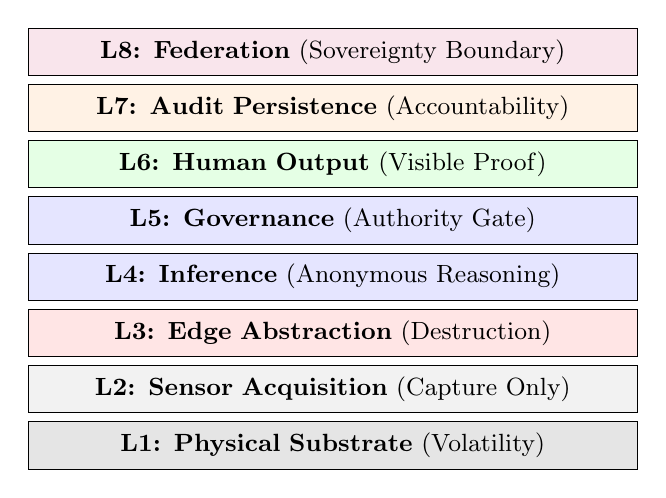
\begin{tikzpicture}[
    node distance=0.5cm,
    layer/.style={rectangle, draw, fill=white, text width=7.5cm, minimum height=0.6cm, align=center, font=\small},
    group/.style={rectangle, draw=gray, dashed, inner sep=0.2cm}
]

\node[layer, fill=purple!10] (L8) {\textbf{L8: Federation} (Sovereignty Boundary)};
\node[layer, fill=orange!10, below=0.1cm of L8] (L7) {\textbf{L7: Audit Persistence} (Accountability)};
\node[layer, fill=green!10, below=0.1cm of L7] (L6) {\textbf{L6: Human Output} (Visible Proof)};
\node[layer, fill=blue!10, below=0.1cm of L6] (L5) {\textbf{L5: Governance} (Authority Gate)};
\node[layer, fill=blue!10, below=0.1cm of L5] (L4) {\textbf{L4: Inference} (Anonymous Reasoning)};
\node[layer, fill=red!10, below=0.1cm of L4] (L3) {\textbf{L3: Edge Abstraction} (Destruction)};
\node[layer, fill=gray!10, below=0.1cm of L3] (L2) {\textbf{L2: Sensor Acquisition} (Capture Only)};
\node[layer, fill=gray!20, below=0.1cm of L2] (L1) {\textbf{L1: Physical Substrate} (Volatility)};

\end{tikzpicture}
\caption{The Canonical Eight-Layer Architecture. Each layer strictly constrains the data available to the layer above it.}
\label{fig:stack}
\end{figure}

\subsection{The Eight Layers as a Closed System}
The canonical eight-layer architecture (Fig. \ref{fig:stack}) is a structural constraint system. Each layer has exactly one role:
\begin{itemize}
    \item \textbf{L1 (Physical Substrate):} Exists to ensure volatility.
    \item \textbf{L2 (Sensor Acquisition):} Exists to capture, not interpret.
    \item \textbf{L3 (Edge Abstraction):} Exists to destroy information.
    \item \textbf{L4 (Inference):} Exists to reason without identity.
    \item \textbf{L5 (Governance):} Exists to decide what may exist beyond the system.
    \item \textbf{L6 (Human Output):} Exists to prove system limits.
    \item \textbf{L7 (Audit Persistence):} Exists to ensure accountability, not recall.
    \item \textbf{L8 (Federation):} Exists to learn without sharing data.
\end{itemize}

% ==========================================
% 6. CANONICAL INVARIANTS AND FORMAL CONSTRAINTS
% ==========================================
\section{Canonical Invariants and Formal Constraints}

The system defines a canonical invariant namespace that establishes irreversibility as a structural property rather than a behavioral expectation. These invariants dictate governance non-bypass as a structural ordering and enforce the federation sovereignty rule.

The primary declarative invariants include:
\begin{itemize}
    \item \textbf{INV-01 (Boundary Irreversibility):} Raw sensor data shall not exist beyond the L3 boundary in any persistent or higher-layer memory region.
    \item \textbf{INV-02 (Data Type Safety):} No RGB or AudioWaveform data types are permitted in L4 memory space. Only KeypointList and SpectralFeatures are valid.
    \item \textbf{INV-03 (Identity Anonymity):} No direct biometric identity representation (e.g., facial imagery, raw audio waveform, persistent identifier token) persists beyond L3.
    \item \textbf{INV-04 (Network Air-Gap):} No external network traffic is permitted from L1-L4 layers. Connectivity is only enabled for L7/L8 via strict proxies.
    \item \textbf{INV-05 (Federation Sovereignty):} Federation cannot transmit raw or pre-boundary data, subject to correct configuration of federation clients and transport layers. 
\end{itemize}

These principles define the architectural doctrine. The full invariant namespace (INV-01 through INV-15), alongside the formal mathematical proofs of their completeness, continuous assertion checks, and implementation-level runtime verification mechanisms, are defined in Paper 18.

% ==========================================
% 7. ETHICAL POSITIONING
% ==========================================
\section{Ethical Positioning and Contribution}

\subsection{From Compliance to Constraint}
Regulatory compliance specifies what should not happen. ScholarMasterEngine specifies what cannot happen. Data minimization, purpose limitation, and the right to erasure are achieved by construction, removing discretion entirely.

\subsection{The Stewardship Model}
This work introduces \textbf{Automated Stewardship} as a distinct ethical category, contrasted with surveillance. Stewardship optimizes harm prevention rather than information extraction, relies on visibility rather than opacity, and constrains direct biometric misuse by removing raw data capability.

\subsection{Ethical Non-Negotiables}
The system is built upon a foundation of ethical non-negotiables that cannot be configured away:
\begin{itemize}
    \item \textbf{No Raw Persistence:} Biometric data never touches non-volatile storage.
    \item \textbf{No Silent Operation:} The system must visibly indicate its state to those being observed.
    \item \textbf{No Pixel-Space Identity Reconstruction:} All output features are abstract and aggregate. This constraint addresses pixel-space reconstruction; dynamic skeletal sequences may carry identity-correlated gait signatures, representing a residual re-identification channel that is acknowledged but outside the scope of this architectural control.
\end{itemize}
These constraints are enforced at compile-time and runtime, not exposed as configuration parameters. This rigidity protects the system against ``mission creep'' and future repurposing.

\subsection{Addressing Common Objections}
A frequent objection to irreversible architectures is the potential for repurposing: ``What if the system is patched to store data?'' Firmware integrity mechanisms (secure boot, kernel lockdown, and read-only overlay filesystems, detailed in Paper 11) may be employed to preserve architectural constraints. Another objection concerns ``Insider Abuse.'' While no system is immune to physical tampering, our ``Separation of Judgment and Authority'' ensures that even an administrator with root access cannot extract raw video because the raw video never reaches persistent storage to begin with.

% ==========================================
% 8. SCOPE & LIMITATIONS
% ==========================================
\section{Limitations, Scope, and Future Directions}
This work is intentionally scoped to educational and campus environments where institutional governance exists. It does not attempt to solve all surveillance contexts or optimize for maximum predictive accuracy at the expense of privacy. By enforcing aggressive abstraction, the system sacrifices fine-grained analysis (e.g., facial expressions).

% ==========================================
% 9. IMPLEMENTATION CONSTRAINTS
% ==========================================
\section{Implementation \& Deployment Constraints}
The theoretical constraints of ScholarMasterEngine rely on specific implementation details. The system requires hardware that supports strict memory isolation to prevent ``data remanence'' attacks. The architecture requires volatile memory zones that prevent persistence; deployment realizations are detailed in Paper 11. Furthermore, sensor isolation protocols ensure that the camera hardware cannot be accessed directly by user-space applications, forcing all data through the abstraction layer (L3). These constraints limit deployment to devices with sufficient control over the hardware-software interface (e.g., NVIDIA Jetson, Raspberry Pi with custom kernels) and preclude use on locked-down consumer mobile operating systems where such low-level control is unavailable.

% ==========================================
% 10. CONCLUSION
% ==========================================
\section{Conclusion}
This capstone has argued that the dominant model of intelligent campus systems---surveillance-first data collection moderated by post-hoc governance---is fundamentally flawed. ScholarMasterEngine demonstrates that an alternative is possible.

By enforcing \textbf{architectural irreversibility}, the system eliminates entire classes of raw-biometric persistence harm before they can arise. By instituting a \textbf{mandatory governance gate}, it ensures that no inference becomes action without explicit ethical scrutiny. By embedding \textbf{visible privacy mechanisms}, it transforms trust from an abstract promise into an observable system behavior.

The eighteen papers comprising the ScholarMaster series form a unified runtime with one data flow, one governance model, and one trust contract. The result is a deployable, verifiable system whose strongest claims can be falsified, audited, and defended.

% ==========================================
% APPENDICES
% ==========================================
\appendices

\section{Paper-to-Layer Traceability}
Table \ref{tab:trace} maps core papers from the ScholarMaster series to the architectural layers they enforce. Note: System-wide integration (P10), Deployment (P11/P12), and Verification (P18) papers span multiple boundaries.

\begin{table}[h]
\caption{System Traceability Matrix}
\centering
\begin{tabular}{p{1.5cm} p{6.5cm}}
\toprule
\textbf{Layer} & \textbf{Associated Papers (ScholarMaster Series)} \\
\midrule
L1: Substrate & P5: Thermal \& Memory Efficiency Benchmarks \\
\midrule
L2: Sensor    & P6: Acoustic Anomaly Detection \\
\midrule
L3: Abstract  & P3: Pose-Only Architectural Irreversibility \\
\midrule
L4: Inference & P1: HNSW Biometric Retrieval Scaling \\
              & P2: Context-Aware Fusion Logic \\
\midrule
L5: Govern    & P7: Spatiotemporal Compliance Verification \\
              & P9: AI Orchestration \& Governance Gates \\
\midrule
L6: Output    & P15: AR-Based Situational Awareness \\
              & P16: Sociological Trust Validation \\
\midrule
L7: Audit     & P8: Trust-Aware Metadata Provenance (Ledger) \\
\midrule
L8: Federation & P13: Intra-Campus Model Drift Compensation \\
               & P14: Sovereignty-Preserving Cross-Campus FL \\
\bottomrule
\end{tabular}
\label{tab:trace}
\end{table}

\section{Canonical Architectural Invariants}
The following invariants define the core structural constraints within the canonical namespace (INV-01 through INV-15):
\begin{itemize}
    \item \textbf{INV-01 (Boundary Irreversibility):} Raw sensor data shall not exist beyond the L3 boundary in any persistent or higher-layer memory region.
    \item \textbf{INV-02 (Data Type Safety):} No RGB or AudioWaveform data types are permitted in L4 memory space. Only KeypointList and SpectralFeatures are valid.
    \item \textbf{INV-03 (Governance Liveness):} Governance Gate status must be ACTIVE. If the policy engine is unreachable, all output ports are disabled.
    \item \textbf{INV-04 (Network Air-Gap):} No external network traffic is permitted from L1-L4 layers. Connectivity is only enabled for L7/L8 via strict proxies.
\end{itemize}

% ==========================================
% REFERENCES
% ==========================================
\begin{thebibliography}{00}

% --- I. Surveillance, Privacy, Trust, and Sociology of AI ---
\bibitem{b1} J. Bentham, \textit{The Panopticon Writings}. Verso, 1995.
\bibitem{b2} D. J. Solove, ``A taxonomy of privacy,'' \textit{Univ. of Pennsylvania Law Review}, vol. 154, no. 3, pp. 477--560, 2006.
\bibitem{b3} S. Zuboff, \textit{The Age of Surveillance Capitalism}. PublicAffairs, 2019.
\bibitem{b4} H. Nissenbaum, \textit{Privacy in Context: Technology, Policy, and the Integrity of Social Life}. Stanford Univ. Press, 2009.
\bibitem{b5} F. Pasquale, \textit{The Black Box Society}. Harvard Univ. Press, 2015.
\bibitem{b6} R. C. Mayer, J. H. Davis, and F. D. Schoorman, ``An integrative model of organizational trust,'' \textit{Acad. of Management Review}, vol. 20, no. 3, pp. 709--734, 1995.
\bibitem{b7} J. D. Lee and K. A. See, ``Trust in automation: Designing for appropriate reliance,'' \textit{Human Factors}, vol. 46, no. 1, pp. 50--80, 2004.
\bibitem{b8} J. Penney, ``Chilling effects: Online surveillance and Wikipedia use,'' \textit{Berkeley Tech. Law Journal}, vol. 31, no. 1, 2016.
\bibitem{b9} R. Benjamin, \textit{Race After Technology}. Polity Press, 2019.
\bibitem{b10} S. U. Noble, \textit{Algorithms of Oppression}. NYU Press, 2018.
\bibitem{b11} V. Eubanks, \textit{Automating Inequality}. St. Martin's Press, 2018.
\bibitem{b12} N. Couldry and U. A. Mejias, ``Data colonialism,'' \textit{Television \& New Media}, vol. 20, no. 4, pp. 336--349, 2019.

% --- II. Cognitive Load, HCI, and Situational Awareness ---
\bibitem{b13} J. Sweller, ``Cognitive load during problem solving,'' \textit{Cognitive Science}, vol. 12, no. 2, pp. 257--285, 1988.
\bibitem{b14} M. R. Endsley, ``Toward a theory of situation awareness,'' \textit{Human Factors}, vol. 37, no. 1, pp. 32--64, 1995.
\bibitem{b15} S. G. Hart and L. E. Staveland, ``Development of NASA-TLX,'' \textit{Advances in Psychology}, vol. 52, pp. 139--183, 1988.
\bibitem{b16} R. R. Hoffman et al., ``Accelerated proficiency and facilitated retention,'' \textit{Cognitive Processing}, vol. 14, no. 2, pp. 147--163, 2013.

% --- III. Augmented Reality, Visualization, and Transparency ---
\bibitem{b18} R. T. Azuma, ``A survey of augmented reality,'' \textit{Presence}, vol. 6, no. 4, pp. 355--385, 1997.
\bibitem{b19} P. Milgram and F. Kishino, ``A taxonomy of mixed reality displays,'' \textit{IEICE Trans. Inf. Syst.}, vol. E77-D, no. 12, pp. 1321--1329, 1994.
\bibitem{b20} D. Schmalstieg and T. H\"ollerer, \textit{Augmented Reality: Principles and Practice}. Addison-Wesley, 2016.
\bibitem{b21} H. Kato and M. Billinghurst, ``Marker tracking for AR,'' \textit{IWAR}, 1999.

% --- IV. Edge AI, Irreversibility, and Privacy by Architecture ---
\bibitem{b23} A. Cavoukian, ``Privacy by design: The 7 foundational principles,'' Information and Privacy Commissioner of Ontario, 2009.
\bibitem{b24} M. Hildebrandt, \textit{Smart Technologies and the End(s) of Law}. Edward Elgar, 2015.
\bibitem{b25} G. Welch and G. Bishop, ``An introduction to the Kalman filter,'' Univ. of North Carolina, 1995.
\bibitem{b26} K. He et al., ``Deep residual learning,'' \textit{CVPR}, 2016.
\bibitem{b27} Z. Cao et al., ``OpenPose: Realtime multi-person 2D pose estimation,'' \textit{CVPR}, 2017.

% --- V. Federated Learning, Differential Privacy, and Sovereignty ---
\bibitem{b28} B. McMahan et al., ``Communication-efficient learning of deep networks,'' \textit{AISTATS}, 2017.
\bibitem{b29} K. Bonawitz et al., ``Practical secure aggregation,'' \textit{ACM CCS}, 2017.
\bibitem{b30} C. Dwork et al., ``The algorithmic foundations of differential privacy,'' \textit{Foundations and Trends in Theoretical CS}, 2014.
\bibitem{b31} T. Li et al., ``Federated learning: Challenges, methods, and future directions,'' \textit{IEEE Signal Processing Magazine}, vol. 37, no. 3, pp. 50--60, 2020.
\bibitem{b32} P. Kairouz et al., ``Advances and open problems in federated learning,'' \textit{Foundations and Trends in ML}, 2021.

% --- VI. Governance, Law, and Compliance ---
\bibitem{b33} European Union, ``General Data Protection Regulation (GDPR),'' Regulation (EU) 2016/679, 2016.
\bibitem{b34} Government of India, \textit{Digital Personal Data Protection Act}, 2023.
\bibitem{b35} K. Crawford and J. Schultz, ``Big data and due process,'' \textit{Boston College Law Review}, 2014.
\bibitem{b36} M. Mitchell et al., ``Model cards for model reporting,'' \textit{FAT '19*}, 2019.

% --- VII. ScholarMaster Series (Primary Sources) ---
\bibitem{b37} N. Babu P., ``Privacy-preserving academic engagement metrics via pose-only architectural irreversibility,'' \textit{ScholarMaster Series}, 2025.
\bibitem{b38} N. Babu P., ``Trust-aware metadata provenance using blockchain,'' \textit{ScholarMaster Series}, 2025.
\bibitem{b39} N. Babu P., ``Context-aware multi-modal inference framework,'' \textit{ScholarMaster Series}, 2025.
\bibitem{b40} N. Babu P., ``Augmented situation awareness using spatially anchored AR,'' \textit{ScholarMaster Series}, 2026.
\bibitem{b41} N. Babu P., ``Beyond the panopticon: Student trust in automated stewardship systems,'' \textit{ScholarMaster Series}, 2026.

% --- VIII. Technical Foundations & Artifacts ---
\bibitem{b42} N. Babu P., ``ScholarMasterEngine,'' GitHub repository, 2025--2026. Available: https://github.com/NarendraaP/ScholarMasterEngine
\bibitem{b43} T. M. Cover and J. A. Thomas, \textit{Elements of Information Theory}. Wiley-Interscience, 2006.
\bibitem{b44} C. E. Shannon, ``A mathematical theory of communication,'' \textit{Bell System Technical Journal}, 1948.


\bibitem{P20} N. Babu P., "Unified Reference Model for ScholarMaster Architecture," \textit{ScholarMaster Series}, 2026.
\bibitem{P21} N. Babu P., "Formal Foundations of Distributed Trust," \textit{ScholarMaster Series}, 2026.
\end{thebibliography}

\end{document}